\documentclass[11pt, a4paper, spanish, openright, twoside]{book}
\usepackage[spanish, activeacute]{babel}
\usepackage[utf8]{inputenc}
%\usepackage[top=2.5cm, bottom=2.5cm, outer=1.75cm, inner=1.75cm, heightrounded, marginparwidth=2.5cm, marginparsep=0.3cm]{geometry}	%márgenes empequeñecidos
\usepackage[top=2.95cm, bottom=2.25cm, outer=2.75cm, inner=2.75cm, heightrounded, marginparwidth=2.5cm, marginparsep=0.3cm]{geometry}	%márgenes originalmente
\usepackage{dpg}
\usepackage{fli}

\usepackage{pgf}
\usepackage{tikz}

\usepgflibrary{shapes.geometric} % LATEX and plain TEX and pure pgf
\usetikzlibrary{arrows,automata,positioning}
\tikzstyle{accepting by double}= [double distance=1.6pt,double,outer sep=.5\pgflinewidth+.8pt] % esto es algo estético.
\renewcommand\shorthandsspanish{}  % para compatibilizar spanish con tikz

%%%%%%		Figuras		%%%%%%%%%%%%%%%%%%%
\usepackage[vflt]{floatflt}		%Entorno float-figure

%%%%%%		Page style		%%%%%%%%%%%%%%%%%%%
\renewcommand{\thepage}{\arabic{page}}% Arabic page numbers\fancyhead{}
\pagestyle{fancy}
\fancyfoot{}
\fancyhead[LO,RE]{Práctica 11}	%encabezado de pares: nombre de la sección
\fancyhead[RO,LE]{Aprendizaje automático con WEKA}
\fancyfoot[LE,RO]{\thepage}	%abajo a izqda en pares, derecha en impares: numero de pagina
%\fancyhead[LE]{\nouppercase{\leftmark}} %cuadro izquierdo de pagina par: parte y contador
\fancyfoot[CE]{Inteligencia Artificial} 
\fancyfoot[CO]{Doble Grado Informática-Matemáticas - Universidad Complutense}
\renewcommand{\footrulewidth}{0.4pt}
\renewcommand{\headrulewidth}{0.4pt}		% linea por debajo del encabezado
\renewcommand{\sectionmark}[1]{\markright{\textbf{\thesection. #1}}}	%negrita
\renewcommand{\labelitemi}{$\circ$} %Primer itemize con circunferencia vacia
\renewcommand{\labelitemii}{$\cdot$} %Segundo itemize con punto pequeño \cdot
\renewcommand*{\thesection}{\arabic{section}}	% Hace que no apareca el indice de capitulos y que comience en section

%%%%%%		Others		%%%%%%%%%%%%%%%%%%%
\setlength{\leftmarginii}{0em} %Segundo itemize sin sangria
\setlength{\leftmarginiii}{1em} %Tercer itemize casi sin sangria
\renewcommand{\labelitemiii}{ }
\pagenumbering{roman}
\addto{\captionsspanish}{\renewcommand*{\contentsname}{Índice}} %Cambia "Indice general" por "Indice"



\begin{document} 
\title{\Huge{\textsc{Inteligencia Artificial}} \\
	\vspace{0.7cm}
	 \textsc{\Large{Práctica 11}} \\
	\vspace{1.5cm}
	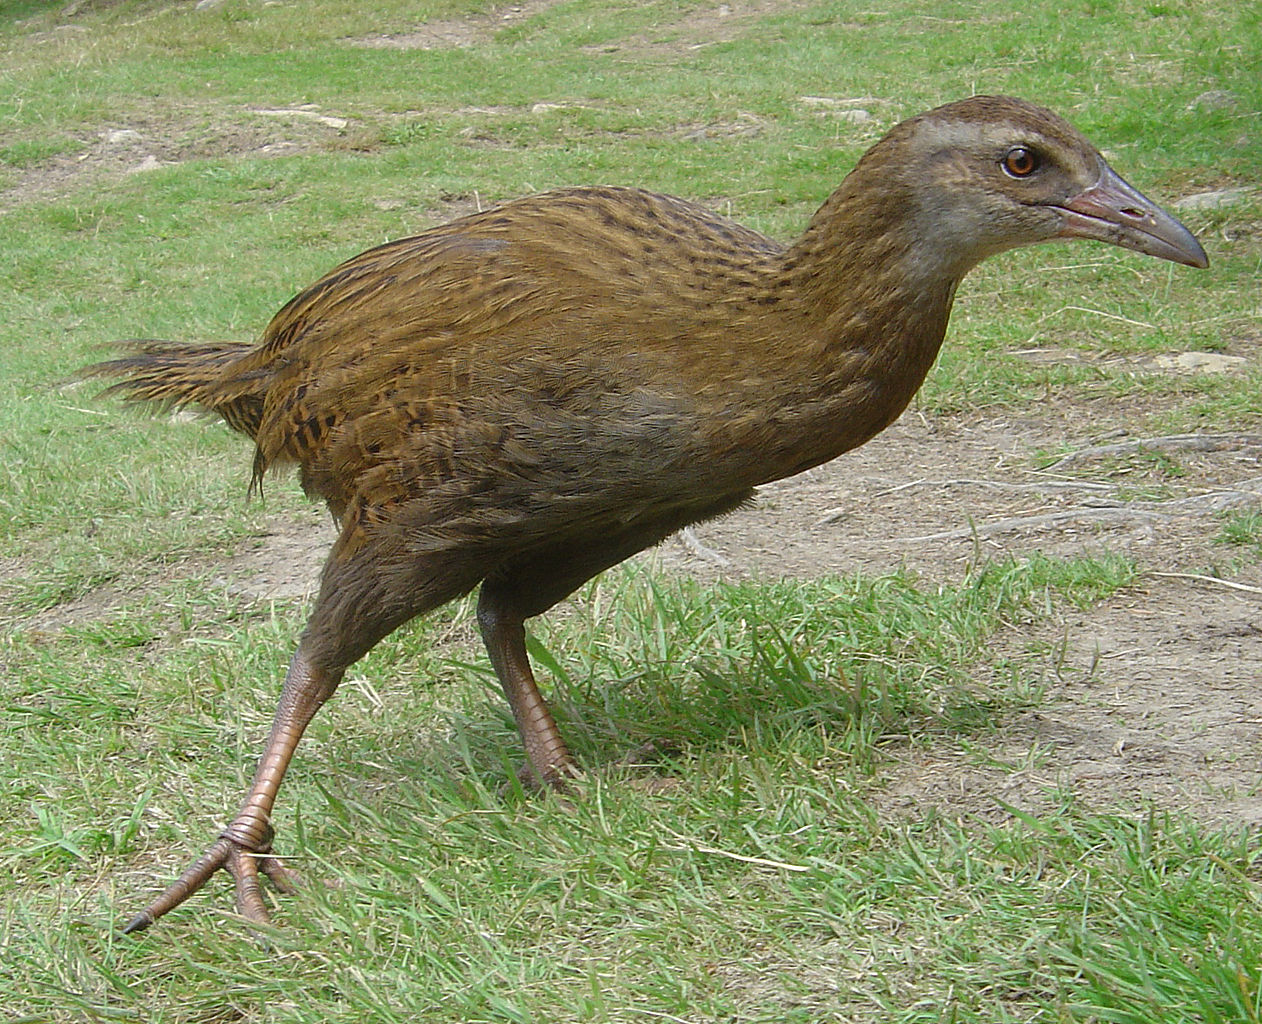
\includegraphics[scale=0.2]{weka}
	}
\author{\textsc{Grupo 3:}\\
	Enrique Ballesteros Horcajo\\
	Ignacio Iker Prado Rujas}
\date{\Today}
\maketitle

\newpage
\mbox{}
\thispagestyle{empty}						% Hoja en blanco, sin numeros ni nada
\newpage


\tableofcontents 							%INDICE hipervinculado

\newpage
\mbox{}
\thispagestyle{empty}						% Hoja en blanco, sin numeros ni nada
\newpage

\pagenumbering{arabic}						% Pone el contador de paginas a 1 y ahora en numeros normales

\vspace{3cm}


\newpage

\begin{section}{Introducción}
	
	En esta práctica vamos a trabajar con el entorno que nos proporciona WEKA\footnote{Página web de WEKA \href{http://www.cs.waikato.ac.nz/ml/weka/}{aquí}.}, aplicando herramientas de aprendizaje automático a conjuntos de datos dados por los ficheros \texttt{diabetes.arff} y \texttt{glass.arff}.
	
\end{section}

\begin{section}{Apartado 1}
	
	\begin{itemize} 
	\item Analiza el archivo citado y contesta las siguientes preguntas: ¿Cuántas instancias hay? ¿Cuántos 
	atributos se utilizan? ¿Por qué atributo queremos aprender a clasificar?

	Hay 768 instancias. Se utilizan 9 atributos, 8 como datos (edad, peso, etc)  y 1 para clasificar (Ser diabético o no). Queremos aprender a clasificar por este último.
 
	\item Ejecuta J48 (versión WEKA de C4.5). Utiliza para la validación el “training set”. Incluye en la 
	memoria los resultados obtenidos y la representación gráfica del árbol correspondiente.


=== Classifier model (full training set) ===

J48 pruned tree
------------------

plas <= 127
|   mass <= 26.4: tested_negative (132.0/3.0)
|   mass > 26.4
|   |   age <= 28: tested_negative (180.0/22.0)
|   |   age > 28
|   |   |   plas <= 99: tested_negative (55.0/10.0)
|   |   |   plas > 99
|   |   |   |   pedi <= 0.561: tested_negative (84.0/34.0)
|   |   |   |   pedi > 0.561
|   |   |   |   |   preg <= 6
|   |   |   |   |   |   age <= 30: tested_positive (4.0)
|   |   |   |   |   |   age > 30
|   |   |   |   |   |   |   age <= 34: tested_negative (7.0/1.0)
|   |   |   |   |   |   |   age > 34
|   |   |   |   |   |   |   |   mass <= 33.1: tested_positive (6.0)
|   |   |   |   |   |   |   |   mass > 33.1: tested_negative (4.0/1.0)
|   |   |   |   |   preg > 6: tested_positive (13.0)
plas > 127
|   mass <= 29.9
|   |   plas <= 145: tested_negative (41.0/6.0)
|   |   plas > 145
|   |   |   age <= 25: tested_negative (4.0)
|   |   |   age > 25
|   |   |   |   age <= 61
|   |   |   |   |   mass <= 27.1: tested_positive (12.0/1.0)
|   |   |   |   |   mass > 27.1
|   |   |   |   |   |   pres <= 82
|   |   |   |   |   |   |   pedi <= 0.396: tested_positive (8.0/1.0)
|   |   |   |   |   |   |   pedi > 0.396: tested_negative (3.0)
|   |   |   |   |   |   pres > 82: tested_negative (4.0)
|   |   |   |   age > 61: tested_negative (4.0)
|   mass > 29.9
|   |   plas <= 157
|   |   |   pres <= 61: tested_positive (15.0/1.0)
|   |   |   pres > 61
|   |   |   |   age <= 30: tested_negative (40.0/13.0)
|   |   |   |   age > 30: tested_positive (60.0/17.0)
|   |   plas > 157: tested_positive (92.0/12.0)

Number of Leaves  : 	20

Size of the tree : 	39
	=== Evaluation on training set ===
	=== Summary ===

Correctly Classified Instances         646               84.1146 %
Incorrectly Classified Instances       122               15.8854 \%
Kappa statistic                          0.6319
Mean absolute error                      0.2383
Root mean squared error                  0.3452
Relative absolute error                 52.4339 \%
Root relative squared error             72.4207 \%
Total Number of Instances              768     

=== Detailed Accuracy By Class ===

               TP Rate   FP Rate   Precision   Recall  F-Measure   ROC Area  Class
                 0.936     0.336      0.839     0.936     0.885      0.888    tested_negative
                 0.664     0.064      0.848     0.664     0.745      0.888    tested_positive
Weighted Avg.    0.841     0.241      0.842     0.841     0.836      0.888

=== Confusion Matrix ===

   a   b   <-- classified as
 468  32 |   a = tested_negative
  90 178 |   b = tested_positive

		\begin{itemize}
			 \item ¿Cuántas instancias han sido mal clasificadas? 122 instancias.
			\item ¿Cuántos nodos terminales hay en el árbol? 20 nodos terminales.
			\item ¿Por qué atributo se clasifica en el primer nivel del árbol? Por plass ( Plasma glucose concentration a 2 hours in an oral glucose tolerance test).
		\end{itemize}

	\item  Vuelve a ejecutar J48 primero con "cross-validation" y después con "percentage split" (con un valor 
	del 66\%) y observa las diferencias. Haz una tabla con el porcentaje de instancias bien clasificadas en 
	cada uno de los tres métodos de validación. Incluye en esa tabla la precisión y el recall para cada 
	uno de los tres métodos.

		\begin{center}
 			 \begin{tabular}{| c | c | c | c |}
 			   \hline
			     				       	  & Training set 	& Cross-validation 		& Percentage splilt  \\ \hline
			    Porcentaje bien clasificadas  	  & 84.1146 \% 	& 73.8281 \%		& 76.2452 \% \\ \hline			 
			    Recall 			     	  & 0.841  		& 0.738 			& 0.762 \\ \hline 
			    Precisión			      	  & 0.842  		& 0.735 			& 0.756  \\ \hline \hline
			    Precisión con negativos		  & 0.839		& 0.790			& 0.809 \\ \hline
			    Precisión con positivos 		  & 0.848 		& 0.632			& 0.644 \\ 
			    \hline
			  \end{tabular}
		\end{center}

		\begin{itemize}
			 \item El porcentaje de bien clasificados es mejor en el primer método ¿Cuál de las tres validaciones te parece 
			más fiable? ¿Por qué? ¿Cuántos falsos negativos (FN) y falsos positivos (FP) se han obtenido con el 
			“percentage split”? 
		\end{itemize}
	

	\end{itemize}
\end{section}

\begin{section}{Apartado 2}
	Para este apartado se utilizará el dataset contenido en el archivo glass.arff incluido en el subdirectorio
	data de la distribución de WEKA y en el campus virtual. Este dataset contiene datos sobre tipos de
	cristal según sus características.

	\begin{itemize}
	\item Analiza el dataset. ¿En cuántas clases se clasifican los ejemplares? ¿Cuántos atributos se utilizan?

	En 7 clases distintas: building windows float processed, building windows non float processed, vehicle windows float  processed,  vehicle windows non float processed, containers, tableware y headlamps.
	Utilizan 9 atributos : RI (refractive index),  Na (Sodium), Mg (Magnesium),  Al (Aluminum), Si (Silicon),  K (Potassium), Ca (Calcium), Ba (Barium) y Fe (Iron). En función de las cantidades para cada cristal se clasificará cada 
	cristal en un tipo de los 7.

	\item Aplica el clustering jerárquico a este conjunto de datos para 7 clusters y comenta los resultados 
	obtenidos. ¿Qué clases han quedado mejor clasificadas?
	Ninguna realmente. Puede decirse que el build wind float y el vehicle wind float son los mejor clasificados porque al menos ha metido todos en el mismo cluster. O que 
	el build wind non-float porque está en el cluster que lleva su nombre. Realmente es una clasificación que no tiene mucha utilidad, pues mete todos en prácticamente la misma clase. 
	Es uno de los problemas que suelen presentarse en  el aprendizaje automático.
	
	\item Discretiza los atributos utilizando un filtro supervisado. ¿Qué horquillas se han generado para los 
	valores del Calcio? Vuelve a ejecutar el clustering jerárquico y compara los resultados con los 
	anteriores. ¿Qué clases han quedado mejor clasificadas?

	Cuatro horquillas: De menos infinito a 7.02, de 7.02 a 8.315, de 8.315 a 10.075 y de 10.075 a infinito.

	Los headlamps han quedado mucho mejor clasificados, pues ahora la mayoría están en una clase propia. Los build wind non-float tienen uno más en "su clase".

	En el resto no hay un cambio significativo.

	\item Con los atributos en su estado original, utiliza el algoritmo de clustering EM (Expectation 
	Maximization) y compara con los resultados anteriores.
	
	Ha mejorado la clasificación de los containers, agrupándolos en una sola clase, pero ha empeorado la clasificación del resto dividiéndolos en distintos clusters.

	¿Qué clases han quedado mejor clasificadas?
	
	Realmente ninguna, los containers los agrupa juntos, pero mete otros tipos de cristales en esa misma clase por lo que tampoco es una clasificación del todo buena.

	¿Qué método de los tres anteriores te parece más útil para este ejemplo? ¿Por qué? 

	Ninguno realmente. El segundo puede ser mejor porque al menos te separa los headlamps y el resto. Sin embargo, ningún método acaba de resultar útil para el ejemplo porque 
	no clasifica bien los tipos de cristales al no ser capaz de distinguir entre ellos y meterlos en la misma clase.

	¿Podríamos haber utilizado un algoritmo de clasificación como J48? 

	Para clasificar por Type desde luego ,  por ejemplo utilizando el 66\% de entrenamiento. Aunque clasifica correctamente solo la mitad de los cristales restantes.

	¿Qué habríamos obtenido con los algoritmos de clustering si no tuviéramos el atributo de clase?

	Agrupa (casi) todos en una misma clase pues no es capaz de encontrar las diferencias sutiles entre los distintos cristales que se dan, y de las que se obtienen las diferentes clasificaciones. 
	No es un problema de relajar las exigencias para cada clase, sino que no sabe qué exigir para poder distinguir unas de otras.

	 ¿En qué casos sólo podríamos utilizar clustering?
	
	Si no tuviésemos las distintas clasificaciones por tipo de cristal, sin ejemplos de entrenamiento, solo podríamos utilizar el clustering para agrupar los cristales en clases diferentes.
	\end{itemize}
\end{section}

	
\begin{thebibliography}{9}

\bibitem{aima}
	Russell, S.; Norvig, P, \\
	\emph{Artificial Intelligence, a modern aproach}.\\
	New Jersey: Pearson, 2010.
	
\bibitem{clase}
	Apuntes y transparencias de Inteligencia Artificial, \\
	Doble Grado Matemáticas - Ing. Informática, U.C.M., 2014-2015.

\end{thebibliography}


\end{document}